\section{My contribution}

\subsection{Introduction}

After outlining the context of the work-study program and describing the technique I worked
on, it is finally time to discuss my contributions to the project. First, I will explore 
the design I implemented and explain why this specific design was chosen. Next, we will 
examine the simulation models I developed and their applications. Following this, I will 
detail the optimization and parallelization of the code that was done to enhance its performance. 
Finally, we will discuss how this optimized code could be utilised to estimate uncertainty
in real-time during synchrotron experiments.

\subsection{Design}

Let us begin the discussion by first looking at the UML diagram of the design (see figure \ref{fig:UML}).

\begin{figure}[h!]
    \centering
    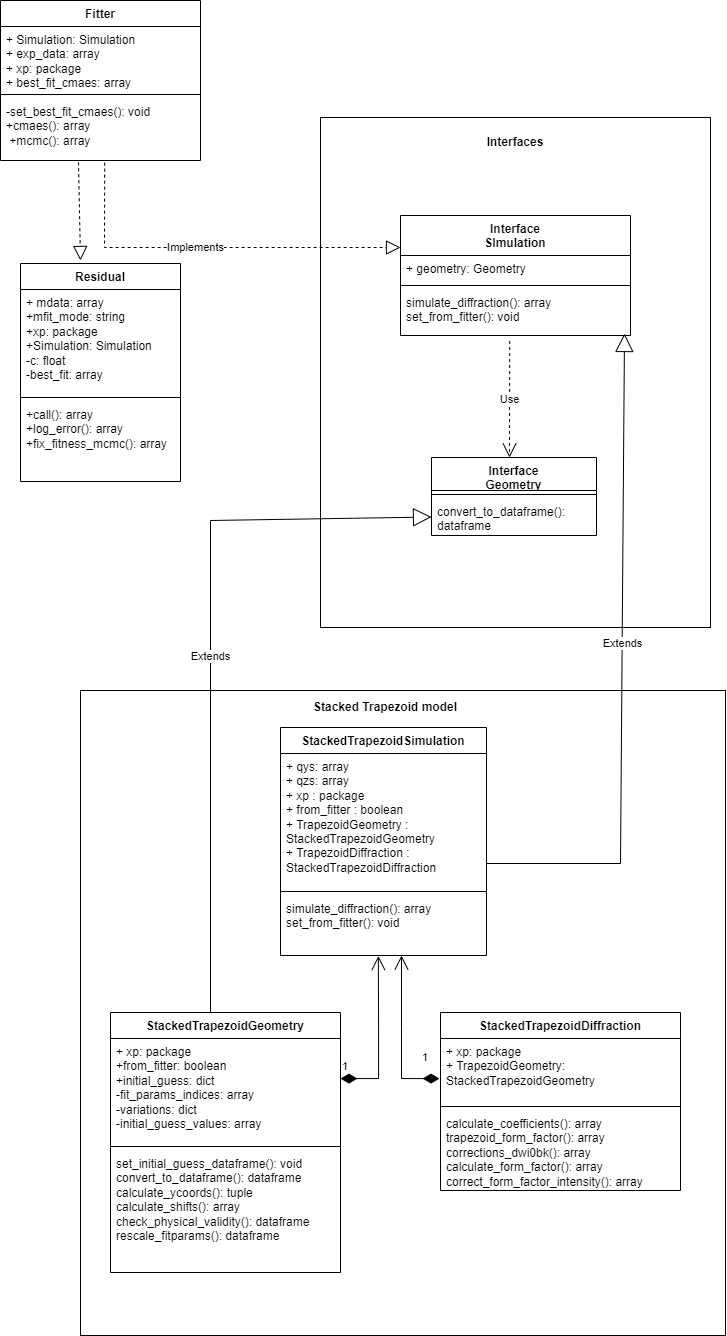
\includegraphics[width=0.7\textwidth]{images/cdsaxs_UML.png}
    \caption{UML diagram of the design for CD-SAXS simulation application. }
    \label{fig:UML}
\end{figure}


\subsection{Simulation Models}
\subsection{Optimisation and parrellelisation}
\subsection{On the fly uncertainity estimation}